\begin{table*}[t]
\centering
\small
\begin{minipage}{0.48\textwidth}
\centering
\textbf{Training tasks}\\[2pt]
\begin{tabular}{lrrr}
\toprule
Website & No rules & \expel{}-style & Reflection \\
\midrule
V1.45.0 & 9/68 & 56/68 & -- \\
V2 & -- & 60/68 & 67/68 \\
V3 & -- & 8/68 & 65/68 \\
\bottomrule
\end{tabular}
\end{minipage}
\hfill
\begin{minipage}{0.48\textwidth}
\centering
\textbf{Held-out validation tasks}\\[2pt]
\begin{tabular}{lrrr}
\toprule
Website & No rules & \expel{}-style & Reflection \\
\midrule
V1.45.0 & 133/167 & 124/167 & -- \\
V2 & -- & 114/167 & 143/167 \\
V3 & -- & 66/167 & 97/167 \\
\bottomrule
\end{tabular}
\end{minipage}
\caption{Overall success counts across website versions. \expel{}-style rules help on \linkding{} V1.45.0 but degrade under harder website drift. Reflection rules remain stronger on the generated website suites. Detailed per-drift results for R1--R4 on website V3 are reported in Appendix Tables~\ref{tab:training_v3_appendix} and~\ref{tab:heldout_v3_appendix}.}
\label{tab:website_version_summary}
\end{table*}

\begin{figure*}[t]
\centering
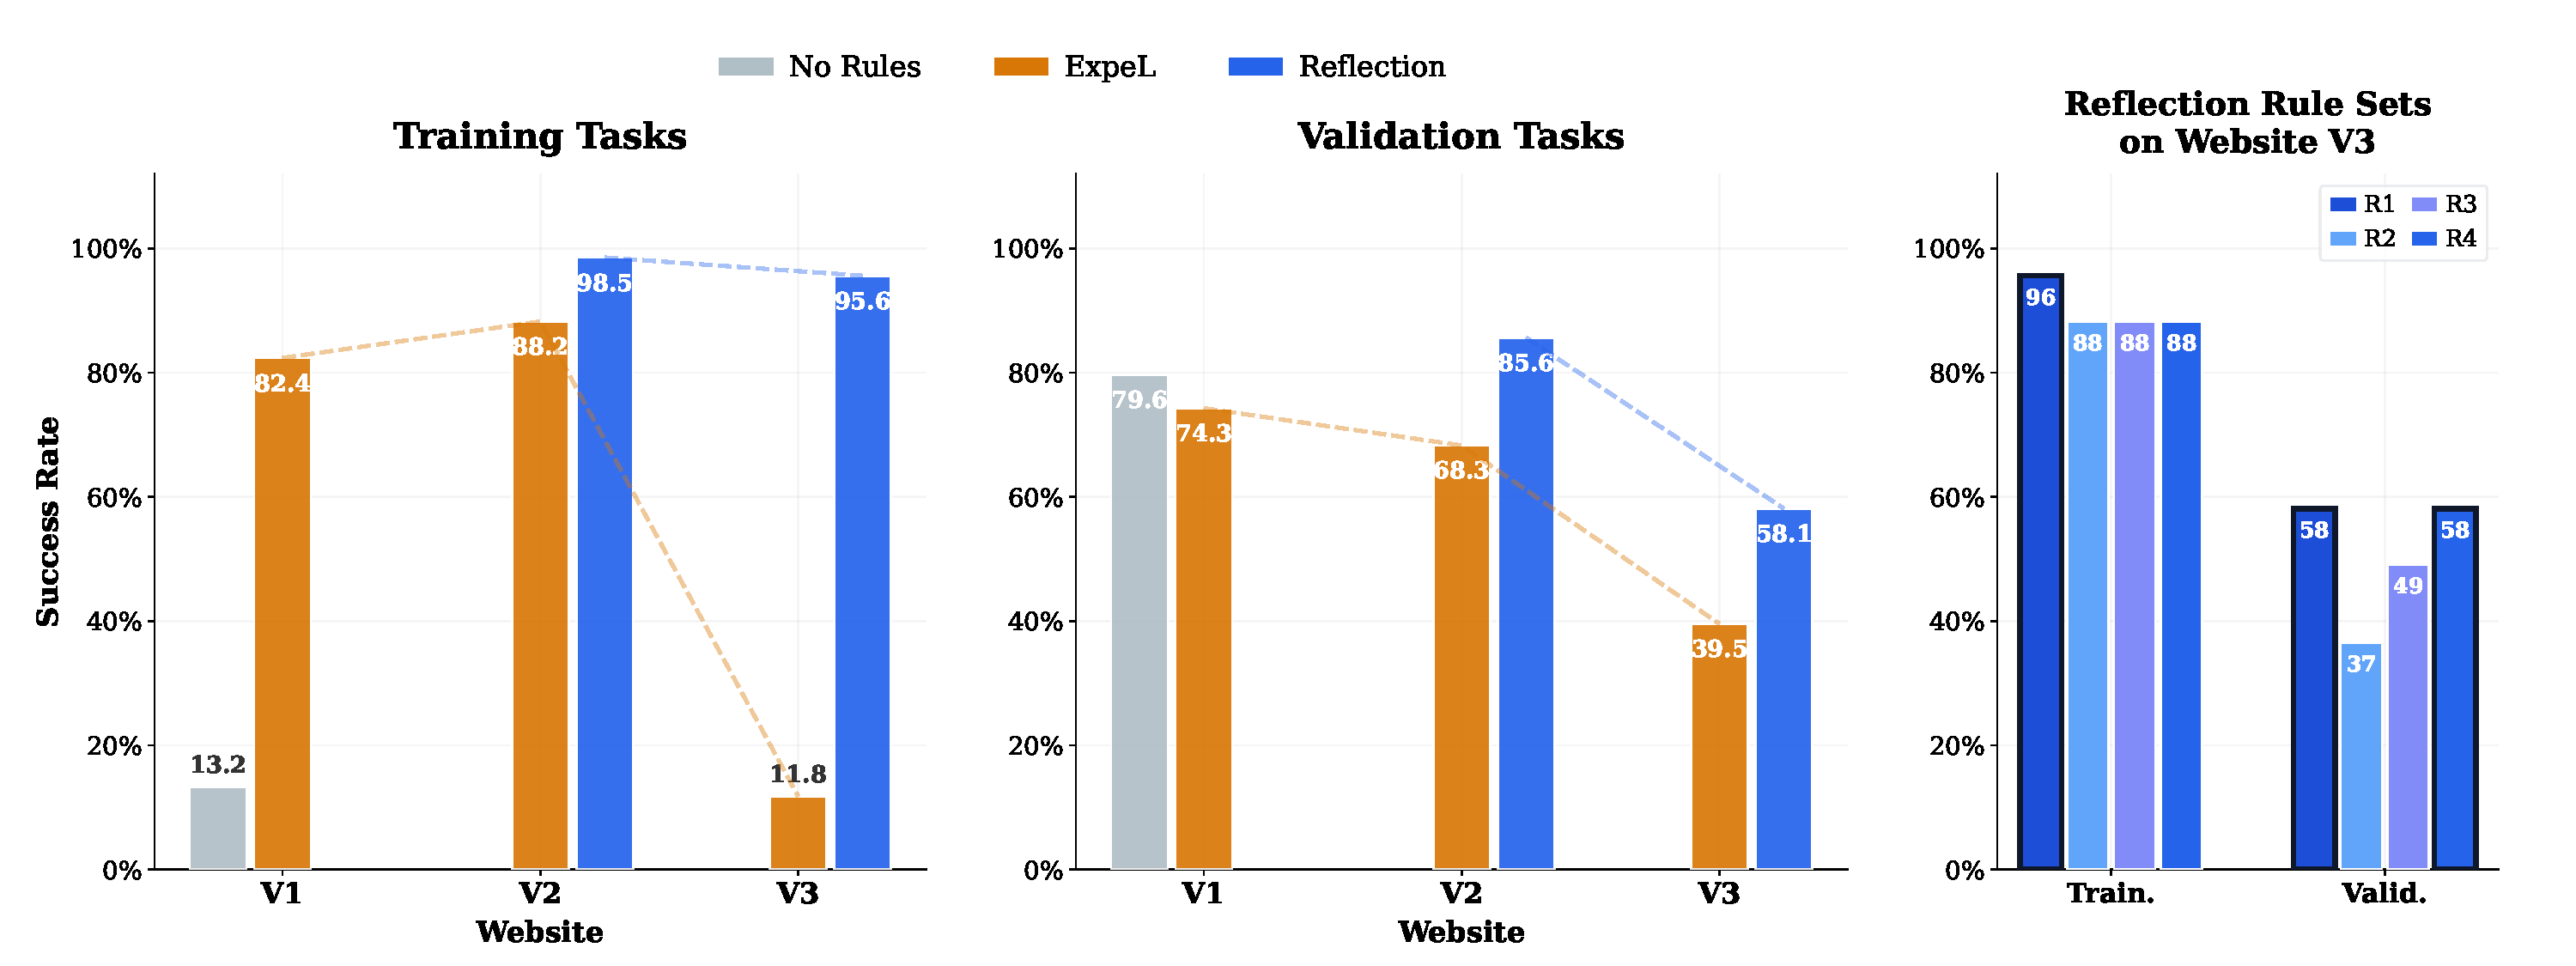
\includegraphics[width=\textwidth]{output/poster_fig_a_hero.pdf}
\caption{Headline robustness results across website versions. The left and middle panels compare no rules, \expel{}-style rules, and the strongest available reflection-rule condition on the training and held-out validation tasks. The right panel isolates the website V3 reflection-rule sets R1--R4, showing that later rule revisions are not monotonically better.}
\label{fig:website_version_overview}
\end{figure*}

\begin{table}[t]
\centering
\small
\begin{tabular}{lcc}
\toprule
Rules & Training & Held-out \\
\midrule
R1 & 65/68 (95.6\%) & 97/167 (58.1\%) \\
R2 & 60/68 (88.2\%) & 97/167 (58.1\%) \\
R3 & 60/68 (88.2\%) & 61/167 (36.5\%) \\
R4 & 60/68 (88.2\%) & 82/167 (49.1\%) \\
\bottomrule
\end{tabular}
\caption{Overall website V3 success for successive reflection-rule sets. R1--R4 are obtained through iterative reflection on observed failures and rule revision; detailed per-drift counts are deferred to Appendix Tables~\ref{tab:training_v3_appendix} and~\ref{tab:heldout_v3_appendix}.}
\label{tab:v3_reflection_overall}
\end{table}
